\documentclass{article}

% Gives us lovely headers
\usepackage{fancyhdr}

% Gives us bigger margins on the right (and smaller on the left) for the margin
% paragraphs
\usepackage[left=2cm,
			top=1.5cm,
			right=5cm,
			bottom=2cm,
			marginparwidth=4cm,
			marginparsep=3mm]{geometry}
% Lets us set the author and title of the compiled pdf file
\usepackage[pdftex]{hyperref}

% Import the packages for the notes
% For line brakes in tables
\usepackage{tabularx}
% For the split environment
\usepackage{amsmath}
% For tabs in verbatim
\usepackage{moreverb}
% For drawing stacks
\usepackage{drawstack}

% Set the author and title
\newcommand{\Author}{Todd Davies} 
\newcommand{\Title}{COMP12111 notes}

% Meta
\author{\Author}
\title{\Title}
% Meta
\author{\Author}
\title{\Title}

% Means that I don't have to type \marginpar{\raggedright \scriptsize every 
% time I want a margin paragraph
\makeatletter
\renewcommand{\@marginparreset}{%
  \reset@font\scriptsize
  \raggedright
  \@setminipage
}
\makeatother

\begin{document}
% Set the headers
\rhead{\title}
\chead{}

% Make the title page(s) centered
\newgeometry{left=2cm,
			top=1.5cm,
			right=2cm,
			bottom=2cm,
			marginparwidth=0cm,
			marginparsep=0mm}

\maketitle

% Get the course info
\courseinfo
\newpage

\tableofcontents
\newpage

% Restore the extra margin geometry
\restoregeometry

% Set the author and title of the compiled pdf
\hypersetup{
	pdftitle = {\Title},
	pdfauthor = {\Author}
}

\section{Introduction}
\subsection{A Computational Model}

The simplest, earliest, commonest, most important computational model is the
\textbf{Von-Neumann Imperative Procedural Computer Model}

According to this model, a computer can:
\begin{enumerate}
	\item Store information
	\item Manipulate the stored information
	\item Make decisions depending on the stored information
\end{enumerate}

\subsection{Simple View Of A Computer}
The simplest model of a computer can be represented as:

\[
	Memory \Leftrightarrow Bus \Leftrightarrow Processor
\]

\subsubsection{Memory}

Memory is a set of locations which can hold information, such as numbers,
programs or many other types of data. Each memory location has a unique
numerical address, and there are typically thousands of millions of different
locations. There are various ways of depicting memory; a common one is a 'hex
dump' that often looks something like this: \marginpar{\raggedright Run the
command {\it hexdump} to generate hexdumps.}

\begin{center}
	\begin{tabular}{l l l}
		{\bf Address}     &	{\bf Hex values}	&	{\bf ASCII}\\
		{\tt 00000000}	&	{\tt 48 65 6C 6C 6F 0A}		&	Hello.\\
	\end{tabular}
\end{center}

Each item that is in the memory has a unique address.

\subsubsection{Bus}

A bus is a bidirectional communication path. It is able to transmit addresses
and numbers between components inside the computer.

\subsubsection{Processor}

The processor obeys a sequence of instructions, commonly referred to as a
program. Historically the processor was often referred to as a CPU, however,
this is inappropriate nowadays since typical processors consist of several
processing cores.

\subsection{Three-address instructions}

Every kind of processor has a different set of instructions, real world examples
include: Pentium, ARM and others

Each three-address instruction:
\begin{enumerate}
	\item Copies the values from any two memory locations and sends them to the processor (source operands)
	\item Copies some operation e.g. adds the copied numbers together
	\item Copies the result back from the processor into a third memory location (destination operand)
\end{enumerate}

For example, if we wanted to convert the Java code {\tt sum = a + b;} into a
three-address instruction we would:

\begin{enumerate}
	\item Identify the two {\it source operands}: $a$ holds 2, $b$ holds 3
	\item Perform the {\it operation}: 2 + 3 = 5
	\item Let the variable $sum$ equal the answer 5. This is the {\it destination operand}
\end{enumerate}

\subsubsection{Three address example}

{\bf Question:} Convert the Java code {\it product = c * d;} into the three-
address style and draw a two box view of it.

First we need to re-write the Java code in the three-address style:
\[
	product \leftarrow c * d
\]
Now we can draw the box view of it (figure~\ref{figure:two_box_model}).

\begin{figure}[ht!]
	\centering
	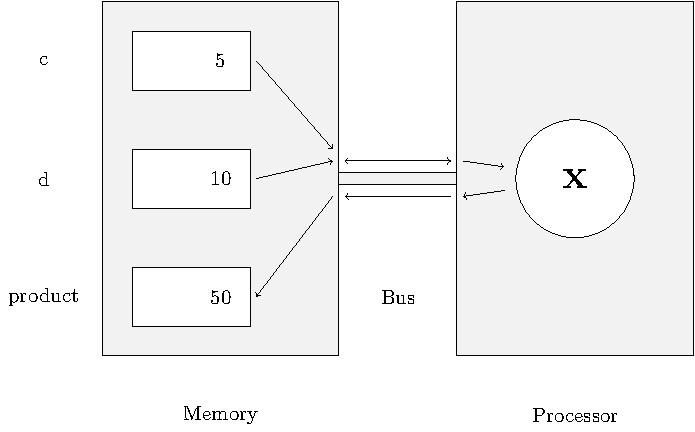
\includegraphics[width=\textwidth]{two_box_model_diagram.pdf}
	\caption{An example of the two box model}
	\label{figure:two_box_model}
\end{figure}

\subsubsection{Memory bottleneck}
Most processors can process instructions faster than they can be fed by memory. Each instruction in the three-address cycle requires four memory cycles:

\begin{enumerate}
    \item Fetch the instruction
    \item Read the first operand
    \item Read the second operand
    \item Write the result to memory
\end{enumerate}

Each of these memory cycles could take hundreds of processor clock cycles to complete, and so in this time the processor would be doing nothing. However, most modern processors employ a {\it cache} to temporarily store commonly accessed memory locations, and so avoid some of the memory cycles. 

\subsection{Registers}
Registers are very small amounts of storage build into a processor. Since they are inside the processor data doesn't need to be transferred over the bus, and so they are very fast. Registers are used instead of the main memory which speeds up program execution.

Each register can only hold one value and each processor will only generally have a few dozen registers (e.g. ARM has sixteen).

\subsection{Instruction Styles}

\subsubsection{One address}
The one address style can only use up to one memory location in each instruction, all other operands must be registers. An example may be:

\[
    R1 \leftarrow R0 + \textrm{\it memory location}
\]

\subsubsection{Load-store}
The load-store style cannot perform operations on memory locations at all. Instead, values from memory must be loaded into a registers before the operation takes place and then the operation can be performed on the registers. Following the operation, the result must be stored back into memory again.

\[
	\begin{split}
	    R1 &\leftarrow \textrm{\it memory location}\\
		R1 &\leftarrow R0 + R1\\
	    \textrm{\it memory location} &\leftarrow R1
    \end{split}
\]

This means that we need extra instructions to do stuff with memory locations:
\begin{enumerate}
	\item \textbf{Load} the value from memory into a register before the operation.
	\item \textbf{Store} the value in the register back to memory after the operation.
\end{enumerate}

For example, the Java code {\it Sum = a + b + c;} would be run as:

\begin{center}
    \begin{tabular}{l l l r}
        R1 & $\leftarrow$ & a & (i.e. load from a)\\
        R2 & $\leftarrow$ & b & (i.e. load from b)\\
        R3 & $\leftarrow$ & R1 + R2 & (i.e. a+b)\\
        R4 & $\leftarrow$ & c & (i.e. load from c)\\
        R5 & $\leftarrow$ & R3 + R4  & (i.e. (a+b)+c)\\
        Sum & $\leftarrow$ & R5 & (i.e. store to sum)\\
    \end{tabular}
\end{center}

You can see that the load-store style favours lots of very simple, very fast instructions.

\section{ARM}
Computers obey programs which are sequences of instructions. Instructions are coded as values in memory. The sequences are held in memory adjacent memory locations. Values in memory can be interpreted as you please, from numbers to text, images or anything really!

Any given set of binary digits can be read as a decimal number, but not always as text, so values in memory are often represented as numbers for convenience.

\subsection{Assembly Language}
Assembly language is a means of representing machine instructions in a human readable form.

Each type of processor has its own assembly language (since each language is
specific to a partiaular architecture) but each instruction typically has a lot
in common:

\begin{itemize}
	\item A mnemonic, that specifies the type of operation
	\item A destination, such as a register or memory location
	\item And one or more sources that may be registers or memory locations.
	\item Possibly with a comment too which will help programmers understand what's happening and aren't interpreted by the assembler.
\end{itemize}

When a program has been written in assembler, it must be {\it assembled} by an {\it assembler} to run it.

\subsection{ARM instructions}

ARM has many instructions but we only need three categories:

\begin{itemize}
	\item Memory operations that move data between the memory and the registers.
	\item Processing operations that perform calculations using value already in registers.
	\item Control flow instructions are used to make decisions, repeat operations etc.
\end{itemize}

\subsection{Transferring data between registers and memory}

Memory operations load a value into a register from an address in memory or
store the value of a register to a memory address.

For example, $a$ into register 1 ($R1 \leftarrow a$) we would write:
{\tt LDR R1, a}

Or to store the value in register 5 into $sum$ ($sum \leftarrow R5$):
{\tt STR R5, sum}

In these examples, $a$ and $sum$ are aliases for the addresses of memory locations.

\subsection{ARM processing instructions}

ARM has many different instructions to perform operations such as addition, subtraction and multiplication.

The syntax for such operations is usually:

\begin{verbatim}
	[operand]	[destination register]	[register 1]	[register 2]
\end{verbatim}

For example, to add two numbers together, we might write:

\begin{verbatim}
	ADD	R2, R0, R1
\end{verbatim}

This will add the value of R0 to the value of R1 and store it in R2.

\subsection{ARM control instructions}

The most common control instruction is the branch. Similar to \texttt{GOTO} in
other languages, a branch will change the PC register (see
section~\ref{subsec:pc}) to another value so the order of execution of the
program is changed.

Branches can be made to be conditional by appending a conditional operator on to
the command.

The syntax is something like:

\begin{verbatim}
	B[conditional operator]	[branch name]
\end{verbatim}

Some examples of different conditional operators are:

\begin{tabularx}{\textwidth}{l X}
	{\bf Command} & {\bf Function}\\
	\texttt{B} & Branches to a different location in the code.\\
	\texttt{BNE} & Branches, but only if the previous condition was false.\\
	\texttt{BEQ} & Branches, but only if the previous condition was true.\\
\end{tabularx}

\subsection{Stored programs and the Program Counter}
\label{subsec:pc}

A computer can make decisions, and choose which instructions to obey next depending upon the results of those decisions. A {\bf Program Counter} (PC) register is used to hold the memory address of the next instruction to be executed. ARM uses register 15 as its PC.

\subsection{Fetch-Execute Cycle}

The processor must first fetch instructions from memory before it can execute them. This is called the fetch-execute cycle, and it involves:

\begin{enumerate}
	\item \textbf{Fetch}: copy the instruction, pointed to by the PC, from memory and set PC to point to the next instruction
	\item \textbf{Execute}:  obey the instruction (exactly as before)
	\item Repeat.
\end{enumerate}

In ARM, the PC starts with a values of \texttt{0x00000000} when the program is initially run. On each cycle of the Fetch-Execute cycle, the PC is incremented by 4, since instructions each occupy 4 memory locations.

\subsection{Decision Making}

In order to make decisions, the computer mustn't just execute instructions one after the other in a linear manner. Instead, branches must be used to change the sequence of instructions to be executed.

In order to perform a conditional branch, we must first perform a compare command to perform the comparison before we do the branch.

\subsubsection{An example}

If we wanted to do a $£1$ discount on a shopping list if the price was over $£20$, we would do the following:

\begin{listing}{1}
		LDR	R0, total	; Load the total price
						; into R0
	
		CMP	R0, #20		; Compare R0 and 20
						; (the literal)
		BLT	nodiscount	; If the price is too low,
						; then don't discount
		SUB	R0, #1		; Deduct £1
		STR	R0, total	; Store the result back 
						; into memory

nodiscount	SVC	2		; Finish

total 		DEFW	25		; Lets say the total is \$25
\end{listing}

\subsection{Allocating memory}

The \texttt{DEFW} (define word) operation puts a value in memory before the program is run. Any define operation is executed before the program is run.

The actual memory location that is used to store the value isn't known to the running program, however, an {\it alias} is attached to the memory location by the programmer and the memory location can be referenced through that.

The syntax for the \texttt{DEFW} command is as follows:

\begin{verbatim}
myage	DEFW	18
\end{verbatim}

Where {\tt myage} is the alias and {\tt 18} is the value.

{\tt DEFW} can also be used to define a number of words:

\marginpar{\raggedright The label is associated with the lowest address (i.e. 0)}
\begin{verbatim}
squares	DEFW	0, 1, 4, 9, 16, 25
\end{verbatim}

{\tt DEFB} stores a single byte in memory. It is useful for strings such as "hello":

\begin{verbatim}
hi	DEFB	"hello"
\end{verbatim}

{\tt DEFS} sets a block of bytes to a set value:

\begin{verbatim}
reserved_space	DEFS	10, 5
\end{verbatim}

The above will set 10 bytes to the value '5'.

\section{Storing values}

% TODO: Expand on this section

There are many ways to store data. For example, we could store what lights are
one in a traffic light in many different ways. First, we must decide how many
different states the traffic light can be in:

\begin{verbatim}
	Red, Red Amber, Green, Amber
\end{verbatim}

You can see that we have four states. This could be represented in binary as two
bits:

\begin{center}
	\begin{tabular}{|c|c|}
		\hline
		{\tt 00} & Red\\ \hline
		{\tt 01} & Red Amber\\ \hline
		{\tt 10} & Green\\ \hline
		{\tt 11} & Amber\\ \hline
	\end{tabular}
\end{center}

We could also store the states as their binary representations of their names:

\begin{center}
	\begin{tabular}{|c|c|}
		\hline
		R & {\tt 01010010}\\ \hline
		RA & {\tt 0101001001000001}\\ \hline
		G & {\tt 01000111}\\ \hline
		A & {\tt 01000001}\\ \hline
	\end{tabular}
\end{center}

You can see though, that this isn't as efficient as storing just two binary
digits.

\section{ARM assembly programming}

\subsection{Different types of values}

ARM has the capacity to work with many different types and sizes of values. Each type has a different use case. The main ones are described below:

\begin{tabularx}{\textwidth}{l l X}
	{\bf Name} & {\bf length} & {\bf Use}\\
	Byte & 8 bits & Used for characters\\
	Word & 32 bits & Used for integer es, addresses and instructions\\
\end{tabularx}

There are other types too (such as the halfword and doubleword) but they aren't needed for this module.

ARM processors require that memory locations are aligned. This means that values stored in memory start at specific places. For example, a word address must be a multiple of four.

This means that after a {\tt DEFW} statement, the {\tt ALIGN} command must be called (See ~\ref{subsubsec:align} for more on the {\tt ALIGN} command.).

\subsection{Loading and storing values in memory}

The commands {\tt LDR} and {\tt STR} are used to move values between memory and registers. The commands are detailed in full below:

\begin{tabularx}{\textwidth}{l X}
	{\bf Command} & {\bf Function}\\
	{\tt STR} & Copies the whole (32 bit) register into memory.\\
	{\tt LDR} & Loads a 32 bit word from memory into a register.\\
	{\tt STRB} & Stores a single 8 bit byte into memory from a register.\\
	{\tt LDRB} & Loads a byte from memory into a register. The upper 24 bits of the register are zeroed.\\
\end{tabularx}

\subsection{Endianness}

Endianness is a property of a memory location that defines the order of the
bits. There are two types of endianness, {\bf little endian} and {\bf big
endian}.

In the word {\tt 0x12345678} there are four bytes:
\begin{itemize}
	\item {\tt 0x12}
	\item {\tt 0x34}
	\item {\tt 0x56}
	\item {\tt 0x78}
\end{itemize}

In little endian, the first byte would be {\tt 0x12} since bits are read from
left to right in little endian.

In big endian, the first byte would by {\tt 0x78} since bits are read from right
to left in big endian.

This is important when we deciding what the most and least significant bits in a
word are. For example, in this instance the {\it lsb} is {\tt 0x12} in little
endian, but {\tt 0x78} in big endian.\marginpar{N.b. The least significant bit
is the smallest address.}

In this course, little endian is used, though ARM can use either.

\subsection{Addressing memory}

ARM uses 32 bit addresses, so there are $2^{32}$ different bytes that can be addressed in memory (or $\frac{2^{32}}{4}$ different words). However, there is no guarantee that the system on which the program is running will have that much memory available.

\subsection{Instruction encoding}

Each ARM instruction is encoded into a four byte word. The exact meaning of each of the bits varies per instruction.

For example, in the branch instruction, the first four bits specify the condition, the second four bits represent the actual operation to perform (i.e. branch) and the remaining twenty four bits define the memory location of the next instruction to branch to.

However, this presents a problem. We only have twenty four bits with which to define the next location to branch to, which allows us to define $2^24$ different locations. However, there are $2^32$ possible addresses that we could use!

This problem is overcome by treating the 24 bits as an offset to the address of the current instruction. This works since most of the time, the address that is being branched to is fairly close to the current instruction.

In order to be able to branch to addresses before and after the current instruction, we must use two's complement to allow signed integers to be used to specify the offset. This means we can branch to any instruction at an address $\pm 2^{23}$ from the current instruction.

\subsection{Literals}

ARM is able to encode literal values into instructions. This saves time having to access registers or memory in order to perform operations such as arithmetic.

An example is to increment a register:

\begin{verbatim}
	ADD	R1, R1, #1
\end{verbatim}

However, ARM only assigns up to 12 bits for a literal value, so we can only have $2^{12}$ values. However, ARM employs a strange method of encoding these values so that more useful values are available (for example, \#512 is allowed, but \#257 isn't).

\subsubsection{Negative literals}

Technically, ARM doesn't support negative literals, however, the assembler will usually be able to find a way to implement them. Some examples are given below:

\marginpar{\raggedright{\tt CMN} is compare negative.\\{\tt MVN} is move not.}
\begin{center}
    \begin{tabular}{l l l r}
        {\tt ADD R1, \#-1} & $\rightarrow$ & {\tt SUB R1, \#1}\\
        {\tt CMP R2, \#-2} & $\rightarrow$ & {\tt CMN R2, \#2}\\
        {\tt MOV R3, \#-3} & $\rightarrow$ & {\tt MVN R3, \#3}\\
    \end{tabular}
\end{center}

\subsection{Supervisor calls}

Supervisor calls are functions implemented by the operating system, not ARM itself. The parameter of an {\tt SVC} call defines it's exact operation.\marginpar{\raggedright SWI is another name for SVC - they do the same thing.}

In this module, the SVC call does the following for each parameter:

\begin{tabularx}{\textwidth}{l X}
	{\tt SVC 0 } & Output a character \\
	{\tt SVC 1 } & Input a character \\
	{\tt SVC 2 } & Stop execution \\
	{\tt SVC 3 } & Output a string \\
	{\tt SVC 4 } & Output an integer \\
\end{tabularx}

\subsection{Pseudo instructions}

The ARM assembler provides some instructions that are translated into sequences of more complicated instructions at the time of assembly for our convenience.

One such instruction is loading a literal into a register. This is done using the {\tt LDR} command as usual, however a literal is used with the '$=$' character instead of a '$\#$'. E.g. to load the value $100$ into register one, we do:

\begin{verbatim}
	LDR	R1,	=100
\end{verbatim}

However, this is a pseudo instruction and will be converted by the assembler to:

\begin{verbatim}
	MOV	R1,	#100
\end{verbatim}

However, if the number is very large, it becomes:

\begin{verbatim}
constant	DEFB	100
		LDR	R1, constant
\end{verbatim}

\subsection{Loading an address into a register}

The {\tt ADR} command loads an address into a register, for example:

\begin{listing}{1}
constant	DEFB	100
		ADR	R1, constant
\end{listing}

Will load the memory address of {\tt constant} into register one.

\subsection{Directives}
Directives are evaluated at the time of assembly.

\subsubsection{DEF commands}

The {\tt DEF\{W,B,S\}} command reserves an amount of memory dependent on the operation used (see the table) and puts an initial value in it.

\begin{tabularx}{\textwidth}{l|X}
	{\bf Command} & {\bf Function}\\ \hline
	{\tt DEFW num} & Reserves a {\it word} of memory and puts the initial value {\tt num} in it.\\ \hline
	{\tt DEFB value} & Reserves {\it byte}(s) of memory and puts the initial value {\tt value} in it. Note that the value can be a string literal, in which case the number of bytes reserved will be equal to the length of the string.\\ \hline
	{\tt DEFS size, fill} & Reserves a {\it block} of memory of {\tt size} bytes and initialises them with the value {\tt fill}. \\ \hline	
\end{tabularx}

\subsubsection{Align}
\label{subsubsec:align}
The align command leaves as many blank bytes as needed so that the next item in memory will start at a word boundary (a multiple of 4).

\subsubsection{Entry}
Sets the PC at the start of the program (i.e. where the program should start from)

\subsubsection{EQU}
Allows you to name a literal, which can go a long way to making the code more maintainable. We could define the literal $18$ as $drinking\_age$:

\begin{listing}{1}
drinking_age	EQU 	#18
		; Check the person is over 18
		CMP 	R1, #drinking_age
		BLT	too_young
\end{listing}

\section{Arithmetic}

\subsection{Making good use of registers}

Registers are a precious resource when programming on ARM. When writing software to evaluate expressions, it's often tempting to load all the variables into registers first, and then perform the arithmetic in separate registers like so:

\begin{listing}{1}
	; a = b + c + d
	LDR 	R1, b
	LDR 	R2, c
	LDR 	R3, d
	ADD 	R4, R1, R2
	ADD 	R5, R4, R3
	STR 	R5, a
\end{listing}

However, this is pointless - the values in the registers {\tt R4} and {\tt R5} aren't going to be needed again, so we may as well do:

\begin{listing}{1}
; a = b + c + d
LDR 	R1, b
LDR 	R2, c
LDR 	R3, d
ADD 	R1, R1, R2
ADD 	R1, R1, R3
STR 	R1, a
\end{listing}

But, we can optimise even further here. Instead of loading all the variables into registers before we do arithmetic, we can save a register and load only the ones we need before each {\tt ADD} instruction:

\begin{listing}{1}
; a = b + c + d
LDR 	R1, b
LDR 	R2, c
ADD 	R1, R1, R2
LDR 	R2, d
ADD 	R1, R1, R2
STR 	R1, a
\end{listing}

Sometimes, it's useful to re-order an arithmetic expression so it can be implemented using less registers. This can often be achieved by increasing the nesting of brackets in an expression such as this:

\[
	(b - e) + (c * d) = ((c * d) + b - e)
\]

Though these expressions are both equal, the right hand side will use a register less in ARM code, since each instruction can be executed sequentially, however the left hand side requires two expressions to be evaluated (and stored in a total of three registers) and then both expressions added together.

\subsection{Using literals in expressions}

If there is a literal in the expression you want to evaluate, then it's possible to use a literal instead of a register. For example, these two programs will end up with the same answer in {\tt R0} but the one on the right uses less registers:

% Split the page into two for side-by-side comparison
\begin{minipage}[t]{0.5\textwidth}
	\begin{listing}{1}
	; (a + 5) * b
	LDR	R0, 5
	LDR	R1, a
	ADD	R0, R0, R1
	LDR	R1, b
	MUL	R0, R0, R1

five	DEFW	5
	\end{listing}
\end{minipage}
\begin{minipage}[t]{0.5\textwidth}
	\begin{listing}{1}
	; (a + 5) * b
	LDR	R0, a
	ADD	R0, R0, #5
	LDR	R1, b
	MUL	R0, R0, R1



	\end{listing}
\end{minipage}

Literals can be any expression that the assembler can evaluate, for example, the following are all valid:\marginpar{\raggedright Note that {\tt MUL} cannot use literals. To get around this, first {\tt MOV} the literal into a register and then multiply.}

\begin{verbatim}
	ADD	R0, R0, #(1 + 2)
\end{verbatim}

% TODO: Check this
\begin{verbatim}
	ADD	R0, R0, #-2
\end{verbatim}

% TODO: Check this
\begin{verbatim}
	ADD	R0, R0, #(2 - 1)
\end{verbatim}

\subsection{Status flags}

ARM has some 1-bit status flags that are set after a {\tt CMP} instruction as shown below:

\begin{tabularx}{0.8\textwidth}{l|X}
	Flag & Meaning\\ \hline
	Negative & Previous result was negative\\ \hline
	Zero & Previous result was zero\\ \hline
	Carry & Previous add or subtract generated a carry\\ \hline
	Overflow & The previous add or subtract overflowed and went out of range\\ \hline
\end{tabularx}

You can get any data operation to alter the flags by appending {\tt S} to the instruction. For example:

\begin{verbatim}
	SUBS	R0, R1, R2
\end{verbatim}

The above command will subtract {\tt R2} from {\tt R1} and store the result in {\tt R0}, but it will also set the flags according to the value of {\tt R0}. For example, if the value in {\tt R0} was negative after the operation, the {\tt Negative} flag would be set.

\subsection{Other useful arithmetic commands}

The {\tt RSB} command is reverse subtract, and is useful for negating a literal:

\begin{verbatim}
	RSB	R1, R0, #0; R1 = 0 - R0 = -R0
\end{verbatim}

The {\tt MLA} command is multiply and add. It can only use registers as operands.

\begin{verbatim}
	MLA	R1, R2, R3, R4 ; R1 = (R2 * R3) + R4
\end{verbatim}

\section{If and While}

\subsection{If statements in ARM}

Given an if statement written in Java such as this:

\begin{listing}{1}
if(condition)
{
    actionStatement;
}
\end{listing}

How would we convert that into ARM assembly? The best way is to do the following:

\begin{enumerate}

	\item Check to see if the condition is else

	\item If it is, then branch to the end of the if statement

	\item Otherwise, perform the action statement

\end{enumerate}

An example implementation may be:

\begin{listing}{1}
	CMP 	R1, R2  ; Compare two registers
	BGE 	endif	; The condition
	MOV 	R1, #0 	; Whatever the action 
					; statement may be
endif
\end{listing}

Note that it is often easier to implement the inverse of some comparisons. For
example, if we were evaluating {\tt (a >= b)} we could do either of these:

\begin{itemize}
	\item 
	\begin{enumerate}
		\item Check whether {\tt a} is greater than {\tt b}
		\item Check whether {\tt a} is equal to {\tt b}
		\item Work out how to branch away if both are false
	\end{enumerate}
	\item 
	\begin{enumerate}
		\item Inverse the comparison and check if {\tt a} is less than {\tt b}
		\item Branch away if it is
	\end{enumerate}
\end{itemize}

\subsection{If else statements}

If else statements are much like if statements, except that if the condition is
false then you branch to the else action, and if the condition is true, then you
branch to after the else statement once you've executed the action. Here's an
example:

Lets implement {\tt if(a==b) { a += 1;} else { b += 1; }}:

\begin{listing}{1}
	LDR 	R0, a
	LDR 	R1, b
	CMP 	R0, R1 	; Compare
	BNE 	else	;If they aren't equal
	ADD 	R0, R0, #1
	B 	end
else 	ADD 	R1, R1, #1
end
\end{listing}

\subsection{While statements}

Implementing a while statement in ARM assembler is very similar to implementing
an if statement, except after you have executed the action statement, you branch
back to the initial condition again, like so:\marginpar{Note that if the code in
your while loop is being executed repeatedly, then it's probably worth
optimising it!}

\begin{listing}{1}
	; Compare two registers
	start	CMP 	R1, R2 
	; The condition
	BGE 	endif
	; Whatever the action statement may be 
	ADD 	R1, R1, #1
	; Branch back to the start
	B	start 
endif
\end{listing}

In ARM, we can make {\it any} instruction have a conditional code on it.
Consequently, we can get rid of a branch instruction, like so:

\begin{listing}{1}
	; Compare two registers
	start	CMP 	R1, R2 
	; Add only if the flag is less than
	ADDLT 	R1, R1, #1 
	; Branch back to the start
	BLT	start
endif
\end{listing}

You can compare the result of an arithmetic instruction with zero by appending
{\tt S} to the instruction like so:

%TODO: Check this
\begin{listing}{1}
start	ADDS 	R0, #1
	BNE 	start
endif
\end{listing}

This will keep adding {\tt 1} to {\tt R0} until it reaches 0. This is often
useful when translating for loops that count up to a number. Instead of counting
up, you can count down using the {\tt SUBS} instruction and only iterate if the
result isn't zero.

\section{Addresses and Addressing}
When a processor references memory it needs to produce an address.

The address needs the same number of bits as the memory address. i.e. 32 in ARM

addressing modes - mechanisms for generating addresses

\subsection{Direct Addressing}
Direct addressing is a mode where the address is simply contained within the instruction.

This requires an instruction longer than the address size which is a problem because ARMs maximum bit length is 32.

So far, we assumed that direct addressing uses LDR/STR instructions, for example:

\begin{center}
    \begin{tabular}{l l l}
        LDR & R0, & b\\
        LDR & R1, & c\\
        ADD & R0, & R0, R2\\
        STR & R0, & a \\
    \end{tabular}
\end{center}

This looks like direct addressing but on ARM it's 'faked' by the assembler as a pseudo-instruction

\subsubsection{Problems with direct addressing}
ARM: both instructions and addresses are 32 bits, but the instruction also specifies operation so it can't contain every possible address.

Solution: allow a register to contain an address, use the address in the register to do loads and stores.

This is {\bf Register Indirect Addressing}

\subsection{Register Indirect Addressing}
The address is held in the register

It takes only a few bits to select a register (4 bits in the case of ARM R0-R15)

A register can (typically) hold an arbitrary address (32 bits in the case of ARM)

ARM has register indirect addressing

\paragraph{Example}
loading a register from a memory location: LDR R0, b

Could be done using register indirect addressing:

\begin{center}
    \begin{tabularx}{0.8\textwidth}{l l l X}
        ADR & R2, & b & Move the {\bf address} of b into R2\\
        LDR & R0, & [R2] & Use address in R2 to fetch the {\bf value} of b\\
    \end{tabularx}
\end{center}

This is still a bit limited - addresses are:

\begin{itemize}
  \item range limited (within ADR 'instruction')
  \item fixed
\end{itemize}

but:

\begin{itemize}
  \item ADRL pseudo-op allows larger range (at a price)
  \item having addresses a variable once it is often used again
  \item variable are usually 'near' each other
\end{itemize}

\subsubsection{Address Arithmetic}
We can operate on registers, so we can:

\begin{itemize}
  \item store/load/move addresses
  \item do arithmetic to calculate addresses
\end{itemize}

Rather than use e.g. extra ADD instructions, we often use {\bf Base + Offset Addressing} - address addition done within the operand.

We have actually been using this all along: Base = PC register.

\subsection{Offset Addressing}
In offset addressing the address is calculated from a register value and a number.

The register specifier is just a few bits, The offset can be 'fairly small'.

With one register 'pointer' any of several variables in nearby addresses may be addressed.

ARM allows offsets of 12 bits in LDR/STR

These bits can be added or subtracted, for example:

\begin{center}
    \begin{tabular}{l l l}
        {\tt LDR} & R0, & [R1, \#8] \\
        STR & R3, & [R6, \#-0x240]\\
        LDR & R7, & [R2, \#short-constant]
    \end{tabular}
\end{center}

This provides a range of $\pm$ ~4 kilobytes around a 'base' register

In practice this method is adequate for most purposes. 

\section{Strings, bit shifts, rotations and tables}

\subsection{Working with Strings}

A String is just a list of bytes where each byte represents a character. The
last byte in the list is the null byte which contains the value {\tt 0}.

\subsubsection{Loading a String}

In order to load the String into a register, the {\tt ADRL} command must be
used, for example:

\begin{listing}{1}
msg	DEFB 	"My message", 0
	ALIGN

	ADRL 	R0, msg
	SVC 	3
\end{listing}

\subsubsection{Finding the length of a String}

In order to find the length of a String, we need only to loop over each byte in
the String until we get to the null byte, and add up how many iterations we've
done as we go along:

\begin{listing}{1}
	ADRL	R1, message
	MOV 	R2, #0
count 	LDRB 	R0, [R1, R2]
	CMP 	R0, #0
	ADDNE 	R2, R2, #1
	BNE 	count
	STR 	R2, length
\end{listing}

\marginpar{\vspace{-6em}Here, we use {\tt R1} to store the message, {\tt R0} to read each
character, and {\tt R2} to keep the count.}

\subsubsection{Getting the index of a character in a String}

In order to do the equivalent of\\{\tt String.indexOf(character)}, we can do
something similar to finding the length of the String, but we only need to loop
until we get to the character we're looking for.

\begin{listing}{1}
	ADRL	R1, message
	LDRB	R2, character
	count 	LDRB 	R0, [R1] #1
	CMP 	R0, #0
	BEQ 	end
	CMP 	R0, R2
	BNE 	count
	end 	ADRL 	R0, message
	SUB 	R1, R1, R0
	SUB 	R1, R1, #1
	STR 	R0, index
\end{listing}

\marginpar{\vspace{-10em}Note how this snippet has an optimisation to use one less
register during the looping process than the string length snippet does. It
only uses one register to loop over the string and then works out the number of
times it's looped after the character has been found.}

\subsection{Bit shifting and rotations}

Shift operations move all the bits in a word in one direction or another. For
example:

\begin{center}
	\begin{tabular}{|l|c|}
		\hline
		{\bf Shift direction} & {\bf Resultant word}\\ \hline
		No shift & {\tt 10011011}\\ \hline
		Left shift & {\tt 00110110}\\ \hline
		Right shift & {\tt 01001101}\\ \hline
	\end{tabular}
\end{center}

\marginpar{Shifting to the left is like multiplying by two, and shifting to the
right is like dividing by two.}

You might have noticed that a zero is appended to whatever side the bits are
moving away from in order to ensure that the word is still the same number of
bits as before.

Rotation operations are very similar to shift operations, except instead of
padding the word with zeroes, the bit that was lost is appended to the other
side of the word:

\begin{center}
	\begin{tabular}{|l|c|}
		\hline
		{\bf Rotation direction} & {\bf Resultant word}\\ \hline
		No rotation & {\tt 10011011}\\ \hline
		Left rotation & {\tt 00110111}\\ \hline
		Right rotation & {\tt 11001101}\\ \hline
	\end{tabular}
\end{center}

ARM has four different operations for shifting and rotations:

\begin{center}
	\begin{tabularx}{\textwidth}{|l|X|X|}
		\hline
		{\bf Mnemonic} & {\bf Meaning} & {\bf Function}\\ \hline
		{\tt LSL n} & Logical shift left & Shifts left by n bits. Any bits that are lost are zeroed.\\ \hline
		{\tt LSR n} & Logical shift right &  Shifts right by n bits. Any bits that are lost are zeroed.\\ \hline
		{\tt ASR n} & Arithmetic shift right & Shifts right by n bits. Any bits that are lost are set as the sign bit (to preserve the signed bit).\\ \hline
		{\tt ROR n} & Rotate Right & Rotates right by n bits.\\ \hline
	\end{tabularx}
\end{center}

\subsection{Accessing a row in a table}

We can use bit shifts to access a row in a table:

\begin{listing}{1}
	ADRL 	R1, table
	LDR 	R2, [R1, R0, LSL #2]

table 	DEFW 	0
	DEFW 	3
	DEFW 	6
	DEFW 	9
	DEFW 	12
	DEFW 	15
	DEFW 	18
\end{listing}

This snippet will allow us to access the row with an index stored in {\tt R0},
so if {\tt R0} was {\tt 2} then the output in {\tt R2} would be {\tt 6}.

\section{Stacks}

%TODO: Reference STFMD (or whatever it's called)

A stack is a data structure that is used by ARM assembly (an in a variety of
other computing applications) to help maintain the state of a program.

The only operations that can be performed on a Stack are {\tt push} and {\tt
pop}. The former adds an item onto the stack and the latter removes the last
item from the stack. Because these are the only two operations, a Stack is a
type of {\it Last In First Out} data structure.

is usually initialised using the {\tt DEFS} command to reserve a block of space
in memory. This means that the stack will be a fixed size.

In ARM assembly, one register is reserved as the Stack Pointer (SP). This keeps
track of the memory location that addresses the last item in the stack.

Stacks can be implemented where the stack pointer starts at the highest memory
address in the range allocated to the stack, or where it starts at the bottom.
In ARM assembly, it is usual to start the stack pointer at the highest address
and work down.

\subsection{Pushing to a stack}

Lets initialise a stack of five memory locations:

\begin{center}
\begin{drawstack}
	\cell{0}	\cellptr{{\tt 0x00000416}}
	\cell{0}	\cellptr{{\tt 0x00000412}}
	\cell{0}	\cellptr{{\tt 0x00000408}}
	\cell{0}	\cellptr{{\tt 0x00000404}}
	\cell{0}	\cellptr{{\tt 0x00000400}}
\end{drawstack}
\end{center}

The stack pointer will currently be pointed at {\tt 0x00000420}, so the next
stackable memory location will be {\tt 0x00000416}.

If we want to {\it push} an item onto the stack, we need to do two things:

\begin{itemize}

	\item Write the value to the current memory location addressed by the stack pointer.

	\item Decrement the stack pointer by {\tt 4}

\end{itemize}

The ARM command for a stack push is {\tt PUSH}. An example might be:

\begin{verbatim}
	PUSH 	\#20
\end{verbatim}

Or if you wanted to push one or more registers:

\begin{verbatim}
	PUSH 	R1, R2, R3
\end{verbatim}

If we executed the first of these commands ({\tt PUSH \#20}), the stack would
look like this:

\begin{center}
\begin{drawstack}
	\cell{20}	\cellptr{{\tt 0x00000416} (SP)}
	\cell{0}	\cellptr{{\tt 0x00000412}}
	\cell{0}	\cellptr{{\tt 0x00000408}}
	\cell{0}	\cellptr{{\tt 0x00000404}}
	\cell{0}	\cellptr{{\tt 0x00000400}}
\end{drawstack}
\end{center}

Executing {\tt PUSH R2, R3} when the values of {\tt R2} and {\tt R3} were {\tt
523} and {\tt 8} respectively would result in a stack such as:

\begin{center}
\begin{drawstack}
	\cell{20}	\cellptr{{\tt 0x00000416}}
	\cell{523}	\cellptr{{\tt 0x00000412}}
	\cell{8}	\cellptr{{\tt 0x00000408} (SP)}
	\cell{0}	\cellptr{{\tt 0x00000404}}
	\cell{0}	\cellptr{{\tt 0x00000400}}
\end{drawstack}
\end{center}

\subsection{Poping from the stack}

The ARM syntax to pop an item from the stack is very similar. To pop the last
item from the stack into {\tt R1} the command would be:

\begin{verbatim}
	POP 	R1
\end{verbatim}

The stack would now look like:

\begin{center}
\begin{drawstack}
	\cell{20}	\cellptr{{\tt 0x00000416}}
	\cell{523}	\cellptr{{\tt 0x00000412} (SP)}
	\cell{8}	\cellptr{{\tt 0x00000408}}
	\cell{0}	\cellptr{{\tt 0x00000404}}
	\cell{0}	\cellptr{{\tt 0x00000400}}
\end{drawstack}
\end{center}

\marginpar{Note that we don't actually have to reset the memory location {\tt
0x00000408} since it will be overwritten on any subsequent push and since the
stack pointer is behind it, it will never be read from.}

And the value of {\tt R1} would be {\tt 8}. This works for multiple registers
too just like the {\tt PUSH} command does.

\subsection{Other ways of accessing the stack}

It's important to remember that the stack is just a set of memory locations, and
the stack pointer is just a normal register. This means that other commands for
accessing memory can also be used to access and manipulate the stack. For
example, take a look at this block:

\begin{listing}{1}
	LDR 	R1, SP
	ADD 	SP, SP, #4
\end{listing}

\marginpar{Of course, we could use post indexed addressing in order to do the
same thing: {\tt LDR R1, [SP], \#4}}

This will load the value of the memory location addressed by the value inside
the stack pointer into {\tt R1} and then increment the stack pointer by 4.
Essentially, this is doing the same thing as {\tt POP R1} will do.

In order to do the same thing for pushing to the stack we can do:

\begin{listing}{1}
	SUB 	SP, SP, #4
	STR 	R1, SP
\end{listing}

\marginpar{Which is equal to {\tt STR R1, [SP, \#-4]!}}

\subsection{Stacks and method calls}

It is important that when a program branches from one method to another, the
values stored in the registers are not overwritten for when the program branches
back to the original method.

This problem is resolved by pushing the values stored in the registers onto the
stack before a branch is made, and then poping them off the stack once the
method has finished executing. Alternately, the method that is being called can
preserve the values in the registers by pushing and poping them to and from the
stack at the start and the end of the method. Obviously, only one such method
needs to be employed, so it's best to stick to one convention for the whole
program.

\section{Methods}

The most basic way of calling a method in ARM assembly is by using the {\tt BL}
command. This will do two things:

\begin{enumerate}
	\item Move the current value of the program counter into the link register.
	\item Branch to the label defined in the instruction.
\end{enumerate}

The method being called will use move the value of the link register back into
the program counter once it has finished execution. Here's an example:

\begin{listing}{1}

	start 	B main

add R1R2	ADD 	R1, R1, R2
	; Move the value of the Link
	; Register back into the PC
	MOV 	PC, LR

main 	MOV 	R1, #4
	MOV 	R2, #2
	BL 	addR1R2

\end{listing}

This program will move the values {\tt 4} and {\tt 2} into {\tt R1} and {\tt R2}
respectively, and then branch to a method that will add the two registers
together and store the result in {\tt R1}.

\subsection{Saving the value of registers}

What if a method used lots of registers internally. We should make sure that the
state of the registers is the same at the end of the method as they are at the
start of the method, since otherwise there could be issues with corrupted data.

The easiest way to do this is to stack the parameters, like so:

\begin{listing}{1}
method
	; First lets store the registers
	; we're going to use into memory
	PUSH 	{R0-R2}
	; ===========================
	; Do stuff with the registers
	; ===========================
	POP 	{R0-R2}
	; Branch back to the calling instruction
	MOV 	PC, LR
\end{listing}

\marginpar{If a method calls another method, then the link register will need to
be stacked too!}

\subsection{Passing parameters}

Passing parameters to a method is easy; just add them to the stack! To do this,
just load the variable into a register, then add it to the stack:

\begin{listing}{1}
	LDR 	R0, myvar
	STR 	R0, [SP,#-4]!
\end{listing}

When the method wants to access a parameter, it can just load the value in
memory addressed by the stack pointer, adding an offset of {\tt \#4} if the
second parameter needs to be accessed, {\tt \#8} for the third and so on. If the
fourth parameter was to be loaded, then the instruction would be {\tt LDR R0
[SP, \#12]}.

\subsection{Stack frames}

A stack frame is a set of stacked values that are related to a particular method
call. They usually have a format that is specific to the method being called.
For example:

\begin{center}
\begin{drawstack}
	\cell{Method variables}	\cellptr{{\tt SP}}
	\cell{Callee saved registers}
	\cell{LR}
	\cell{Parameters}
	\cell{Caller saved registers}
\end{drawstack}
\end{center}

\section{Switch statements}
\label{sec:switch}
Obviously, a switch statement could be compiled down to a series of {\tt if
else} statements and then converted into ARM assembly. However, if we had a long
list of conditions, and our condition was either near the bottom of the list, or
maybe even the {\tt default} choice, then we'd need to test the switch
expression against all of the conditions before being able to decide what to do.

This has the potential to be very inefficient, so thankfully, there is another
way to do it. We can use the value of the switch variable to branch directly to
the piece of code that we want to execute for that case.

This can be achieved using a table of values where the offset in the table
corresponds to the next address to load into the PC (i.e. the branch location).
For example:

\marginpar{\vspace{8em} The {\tt LSL} command is used to shift the bits in {\tt
R1} left. The number of places shifted is equal to the value of {\tt R0}. This
has the effect of adding {\tt (4*R0)} onto {\tt R1}.}

\begin{listing}{1}
; Define a table of variables with 
; the locations to branch to
swtable	DEFW	case0
	DEFW 	case1
	DEFW 	default
	DEFW 	case2
; Load the base address of the table
; into R1
	ADR 	R1, swtable
; Load the value of R1 into the PC.
; Offset the value in R1 by (R0*4)
	LDR 	PC, [R1, R0, LSL, #2]

case0	; Do stuff
	B end

case1	; Do stuff
	B end

case2	; Do stuff
	B end

default	; Do stuff
	B end
\end{listing}

It's important to catch cases where the expression isn't in the table too, for
example, if (following the previous example) the values we wanted to implement
specific logic for were {\tt (0, 1, 3)}, then we would need to catch cases where
the value was less than {\tt 0} and greater than {\tt 3}.

\begin{listing}{1}
	CMP 	R0, #0
	BLT 	default
	CMP 	R0, #3
	BGT 	default
\end{listing}

The above would go before the table lookup would occur.

\section{Types of values}

\subsection{Signed and unsigned integers}

Lets assume that integers only have 8 bits, and so can hold $2^8$ ($256$)
different values. If we use a signed integer, the most significant bit would
indicate whether the number was negative or not. This means that we loose a
bit's worth of data and therefore can only represent the numbers $0-128$, though
we do gain the ability to distinguish negative numbers from positive numbers.

\marginpar{As you should already know, using a signed integer is also known as
2's complement.}

Note that the numbers $0-127$ are represented as the same as both signed and
unsigned integers, however, when a number reaches the value $128$, then as a
signed integer it would mean $-1$ and as an unsigned integer it would mean
$128$.

It is important to note, that ARM has different types of compare instructions
for signed and unsigned integers. We can use this to our advantage in the switch
example outlined in the previous section (see page~\pageref{sec:switch}).

If we treat the register {\tt R0} as a signed integer, we will have to check
whether it is below {\tt 0} and whether it's above {\tt 4}. However, if we use
unsigned comparisons, we only need to check whether the register is above {\tt
4} since any negative value will be represented as a positive value much larger
than {\tt 4}!

\begin{listing}{1}
	CMP 	R0, #4
	BHI 	default
\end{listing}

\subsection{Booleans in ARM assembly}

Since a boolean value is either true or false, it is obvious that we only need a
minimum of one bit to represent it. However, due to the difficulties of
accessing just one bit in the ARM architecture, it actually make more sense to
represent a boolean as a byte, where the least significant bit is either {\tt 1}
or {\tt 0} depending on the value of the boolean.

This is easy, since it means that booleans are represented as the integers {\tt
0} and {\tt 1}. Testing a boolean value is easy too, since all you need to do is
compare it to zero or one.

\begin{verbatim}
	CMP 	R1, #0
\end{verbatim}

\subsubsection{Logical operators in ARM}

ARM assembly implements four logical operators:

\begin{itemize}

	\item {\tt AND} (logical AND)
	\item {\tt ORR} (logical OR)
	\item {\tt EOR} (logical XOR)
	\item {\tt BIC} (bit clear)
	\item {\tt MVN} (logical not)

\end{itemize}

All of these are self explanatory except from the bit clear one, which is
explained using a table:

\begin{tabular}{|c|c|c}

	A & B & BIC A B\\ \hline
	0 & 0 & 0\\
	0 & 1 & 0\\
	1 & 0 & 1\\
	1 & 1 & 0\\
	
\end{tabular}

{\tt BIC} is equivalent to {\tt A \& !B}. If {\tt B} is high, then the output will
be {\tt 0}, otherwise, it will be {\tt A}.


\end{document}